% \documentclass{standalone}
% \usepackage[dvipsnames]{xcolor}
% \usepackage{tikz}
\usetikzlibrary{arrows.meta}

% \begin{document}
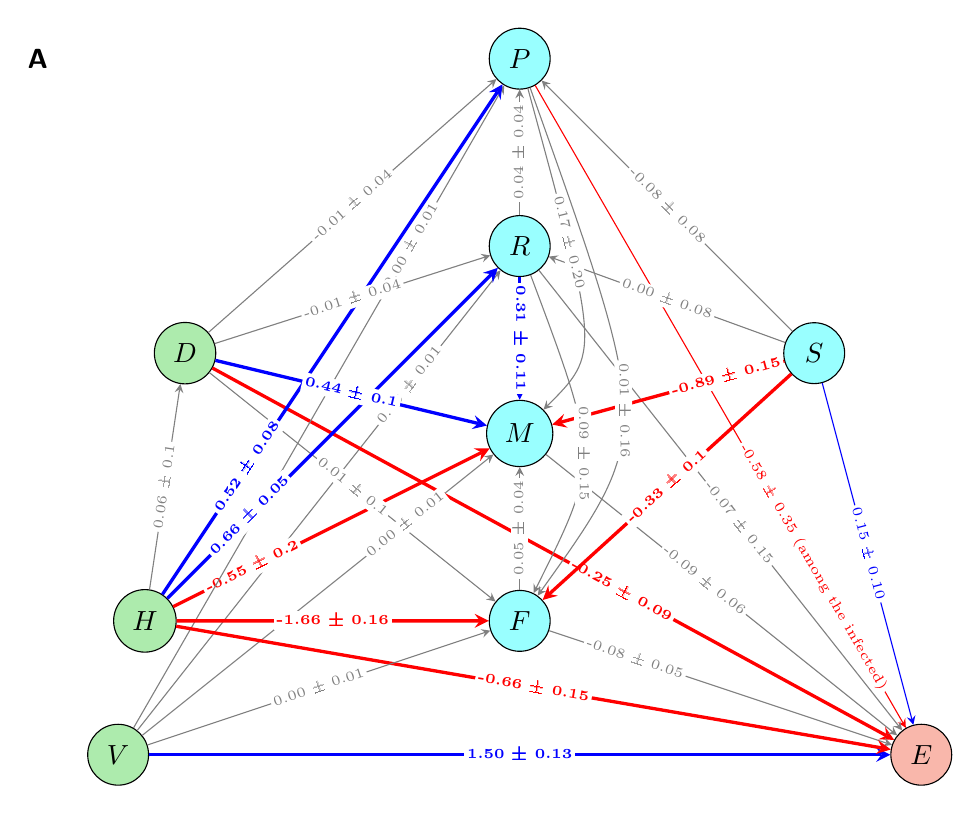
\begin{tikzpicture}[scale=1.7]
	\node[inner sep = 0, font=\sffamily] (panel A) at (-3.6,5.2) {\textbf{A}};
	\node[circle, draw, inner sep=4pt, fill=LimeGreen, font=\bfseries, text opacity=1, fill opacity=0.4, minimum width=22pt] (V) at (-3,0) {\(V\)};
	\node[circle, draw, inner sep=4pt, fill=RedOrange, font=\bfseries, text opacity=1, fill opacity=0.4, minimum width=22pt] (E) at (3,0) {\(E\)};
	\node[circle, draw, inner sep=4pt, fill=LimeGreen, font=\bfseries, text opacity=1, fill opacity=0.4, minimum width=22pt] (H) at (-2.8,1) {\(H\)};
	\node[circle, draw, inner sep=4pt, fill=LimeGreen, font=\bfseries, text opacity=1, fill opacity=0.4, minimum width=22pt] (D) at (-2.5,3) {\(D\)};
	\node[circle, draw, inner sep=4pt, fill=Cyan, font=\bfseries, text opacity=1, fill opacity=0.4, minimum width=22pt] (F) at (0,1) {\(F\)};
	\node[circle, draw, inner sep=4pt, fill=Cyan, font=\bfseries, text opacity=1, fill opacity=0.4, minimum width=22pt] (M) at (0,2.4) {\(M\)};
	\node[circle, draw, inner sep=4pt, fill=Cyan, font=\bfseries, text opacity=1, fill opacity=0.4, minimum width=22pt] (R) at (0,3.8) {\(R\)};
	\node[circle, draw, inner sep=4pt, fill=Cyan, font=\bfseries, text opacity=1, fill opacity=0.4, minimum width=22pt] (P) at (0,5.2) {\(P\)};
	\node[circle, draw, inner sep=4pt, fill=Cyan, font=\bfseries, text opacity=1, fill opacity=0.4, minimum width=22pt] (S) at (2.2,3) {\(S\)};

	\draw [-stealth, gray] (V) -- (R) node[near end, font=\tiny,
		fill=white, sloped, inner sep=1] {0.00 ± 0.01};
	\draw [-stealth, red, very thick] (H) -- (M) node[near start, font=\tiny\bfseries, text=red,
		fill=white, sloped, inner sep=1] {-0.55 ± 0.2};
	\draw [-stealth, red, very thick] (D) -- (E) node[pos=0.6, font=\tiny\bfseries, text=red,
		fill=white, sloped, inner sep=1] {-0.25 ± 0.09};
	\draw [-stealth, gray] (D) -- (F) node[midway, font=\tiny,
		fill=white, sloped, inner sep=1] {0.01 ± 0.1};
	\draw [-stealth, gray] (D) -- (P) node[midway, font=\tiny,
		fill=white, sloped, inner sep=1] {-0.01 ± 0.04};
	\draw [-stealth, gray] (F) -- (E) node[near start, font=\tiny,
		fill=white, sloped, inner sep=1] {-0.08 ± 0.05};
	\draw [-stealth, gray] (F) -- (M) node[midway, font=\tiny,
		fill=white, sloped, inner sep=1] {0.05 ± 0.04};
	\draw [-stealth, gray] (M) -- (E) node[pos=0.45, font=\tiny,
		fill=white, sloped, inner sep=1] {-0.09 ± 0.06};
	\draw [-stealth, red] (P) -- (E) node[near end, font=\tiny,
		fill=white, sloped, inner sep=1] {-0.58 ± 0.35 (among the infected)};
	\draw [-stealth, gray] (R) -- (E) node[pos=0.55, font=\tiny,
		fill=white, sloped, inner sep=1] {-0.07 ± 0.15};
	\draw [-stealth, blue, very thick] (R) -- (M) node[midway, font=\tiny\bfseries, text=blue,
		fill=white, sloped, inner sep=1] {0.31 ± 0.11};
	\draw [-stealth, gray] (R) -- (P) node[midway, font=\tiny,
		fill=white, sloped, inner sep=1] {0.04 ± 0.04};
	\draw [-stealth, blue] (S) -- (E) node[midway, font=\tiny,
		fill=white, sloped, inner sep=1] {0.15 ± 0.10};
	\draw [-stealth, red, very thick] (S) -- (F) node[midway, font=\tiny\bfseries, text=red,
		fill=white, sloped, inner sep=1] {-0.33 ± 0.1};
	\draw [-stealth, red, very thick] (S) -- (M) node[near start, font=\tiny\bfseries, text=red,
		fill=white, sloped, inner sep=1] {-0.89 ± 0.15};
	\draw [-stealth, gray] (S) -- (P) node[midway, font=\tiny,
		fill=white, sloped, inner sep=1] {-0.08 ± 0.08};
	\draw [-stealth, gray] (S) -- (R) node[midway, font=\tiny,
		fill=white, sloped, inner sep=1] {0.00 ± 0.08};
	\draw [-stealth, gray] (V) -- (M) node[near end, font=\tiny,
		fill=white, sloped, inner sep=1] {0.00 ± 0.01};
	\draw [-stealth, gray] (V) -- (P) node[near end, font=\tiny,
		fill=white, sloped, inner sep=1] {0.00 ± 0.01};
	\draw [-stealth, blue, very thick] (V) -- (E) node[midway, font=\tiny\bfseries, text=blue,
		fill=white, sloped, inner sep=1] {1.50 ± 0.13};
	\draw [-stealth, gray] (H) -- (D) node[midway, font=\tiny,
		fill=white, sloped, inner sep=1] {0.06 ± 0.1};
	\draw [-stealth, red, very thick] (H) -- (E) node[midway, font=\tiny\bfseries, text=red,
		fill=white, sloped, inner sep=1] {-0.66 ± 0.15};
	\draw [-stealth, red, very thick] (H) -- (F) node[midway, font=\tiny\bfseries, text=red,
		fill=white, sloped, inner sep=1] {-1.66 ± 0.16};
	\draw [-stealth, blue, very thick] (H) -- (P) node[near start, font=\tiny\bfseries, text=blue,
		fill=white, sloped, inner sep=1] {0.52 ± 0.08};
	\draw [-stealth, blue, very thick] (H) -- (R) node[near start, font=\tiny\bfseries, text=blue,
		fill=white, sloped, inner sep=1] {0.66 ± 0.05};
	\draw [-stealth, blue, very thick] (D) -- (M) node[midway, font=\tiny\bfseries, text=blue,
		fill=white, sloped, inner sep=1] {0.44 ± 0.1};
	\draw [-stealth, gray] (R) .. controls (0.6, 2.2) .. (F) node[midway, font=\tiny,
			fill=white, sloped, inner sep=1] {0.09 ± 0.15};
	\draw [-stealth, gray] (P) .. controls (1, 2.4) .. (F) node[midway, font=\tiny,
			fill=white, sloped, inner sep=1] {0.01 ± 0.16};
	\draw [-stealth, gray] (P) .. controls (0.6, 3) .. (M) node[near start, font=\tiny,
			fill=white, sloped, inner sep=1] {0.17 ± 0.20};
	\draw [-stealth, gray] (V) -- (F) node[midway, font=\tiny,
		fill=white, sloped, inner sep=1] {0.00 ± 0.01};
	\draw [-stealth, gray] (D) -- (R) node[midway, font=\tiny,
		fill=white, sloped, inner sep=1] {-0.01 ± 0.04};
\end{tikzpicture}

% \vspace{0.1cm}

\begin{tikzpicture}
	\node[inner sep=0pt, left of = V, align=left] (probs)
	{
\includegraphics[width=0.8\textwidth]{./Figures/plots/MultiLevel_DE_H_E_chn_traces.pdf}};
	\node[inner sep = 0, font=\sffamily, align=left] (panel A) at (-12,4.5) {\textbf{B}};
\end{tikzpicture}
% \end{document}
